\documentclass[a4paper,11pt]{report}
\usepackage{graphicx}
\usepackage{url}
\usepackage[top=1.0in, bottom=1.0in, left=.6in, right=.6in]{geometry}
\usepackage{float}
\addtolength{\topmargin}{-.50in}
\title{Project Reports- CS296 - By Group 12}
\author{Vipul Harsh\\
        110050034\\
        \texttt{vipulharsh.cse.iitb.ac.in}\\[0.3 cm]
        Alok Yadav\\
        110050043\\
        \texttt{yadavalok.iitb.ac.in}\\[0.3 cm]
        Siddhant Mittal\\
        110050015\\
        \texttt{sid@cse.iitb.ac.in}
}

\begin{document}
\maketitle

\section{Introduction}

A Rube Goldberg machine is a deliberately over-engineered or overdone machine that performs a very simple task in a very complex fashion, usually including a chain reaction.\\
\footnote
  { 
 Copied from Wikipedia
 }
In this project , we have attempted to design an Alarm clock on similar lines. When the needle strikes 12 , it triggers a chain of actions ultimately waking up the person. In the following sections , we have further elaborated on our design and the working of the machine.
\\ To achieve the simulation , we've used the Box2d library and GLUI graphics packages.  




\section{Design of the Machine}

Morning Alarm: \\
When the hour's hand hits 12 , the ball(1) gets moving which then falls and hits the pendulums(2) , setting it into motion . \\
    The pendulums(2) goes on to hit the dominos ringing the first bell for the person to wake up. It then hits the ball which then falls on the see-saw tossing the box into the open box(5).The container as a result moves towards the right and the balls fall on the open box(7).The pendulum then pulls the head of the person(8) , forcing it in an upright sitting position.\\
    The person has now gotten out of her sleep.
	
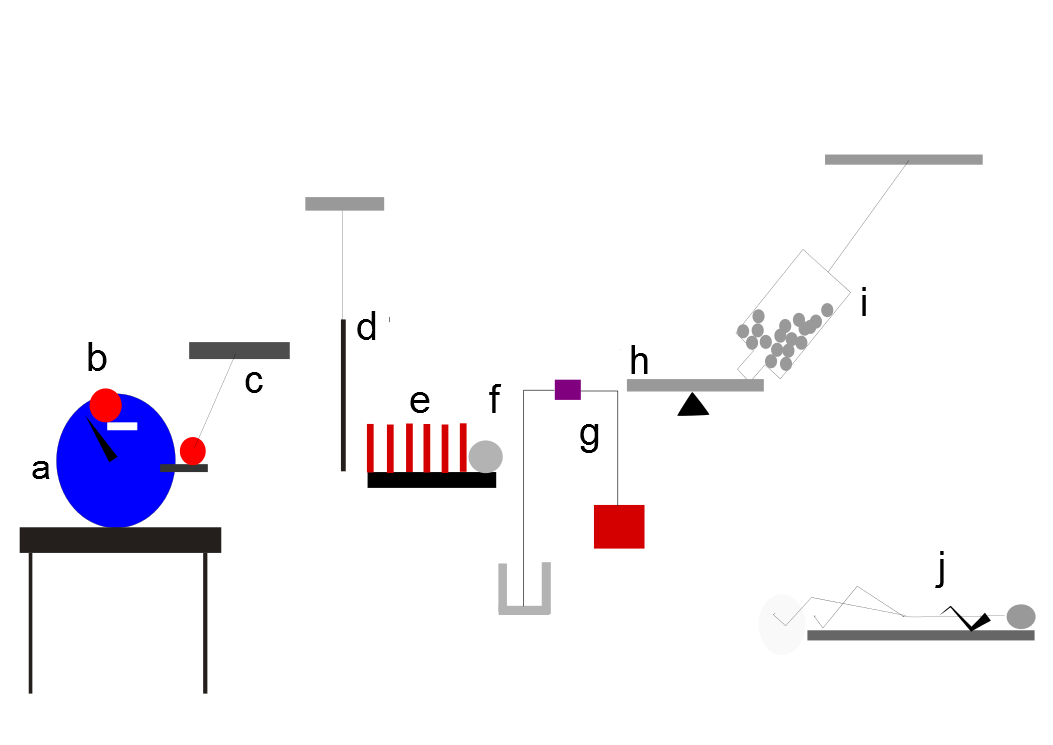
\includegraphics[scale=0.3]{doc/final-design.eps}








\section{Original Design and differences from the original design}

\subsection{Original Design}
When the hour's hand(a) hits 12 , the ball(b) gets moving which then falls and hits the pendulum(c) , setting it into motion . \\
    The pendulum(c) goes on to hit the bell(d), ringing the first bell for the person to wake up. It then hits the ball (e) which then falls on the pendulum (f).
	\\ This throws the rectangular block (g) upwards hitting the seesaw(h) making way for motion of the bottle pendulum(i). Finally the balls fall
	on the sleeping man(j).

\subsection{Differences}
There are some subtle departs from the original design. 
\begin{enumerate}
   \item 
Instead of the rectangular pendulum(d) and the ball(c) , we now have a series of pendulums
   \item
 Instead of the ball(e) straight away falling on the open box(f)  , the ball falls on the see-saw and then 
 a rectangular box(on the other side of the see-saw) goes into the open box setting it into motion  
  \item
 Earlier , the balls in the container(i) fell directly on the person(j). Now the head of the person is tied to the right end of a pulley and the balls fall on the open box to the left of the pulley thereby pulling the person in an upright sitting position.   
 \end{enumerate}

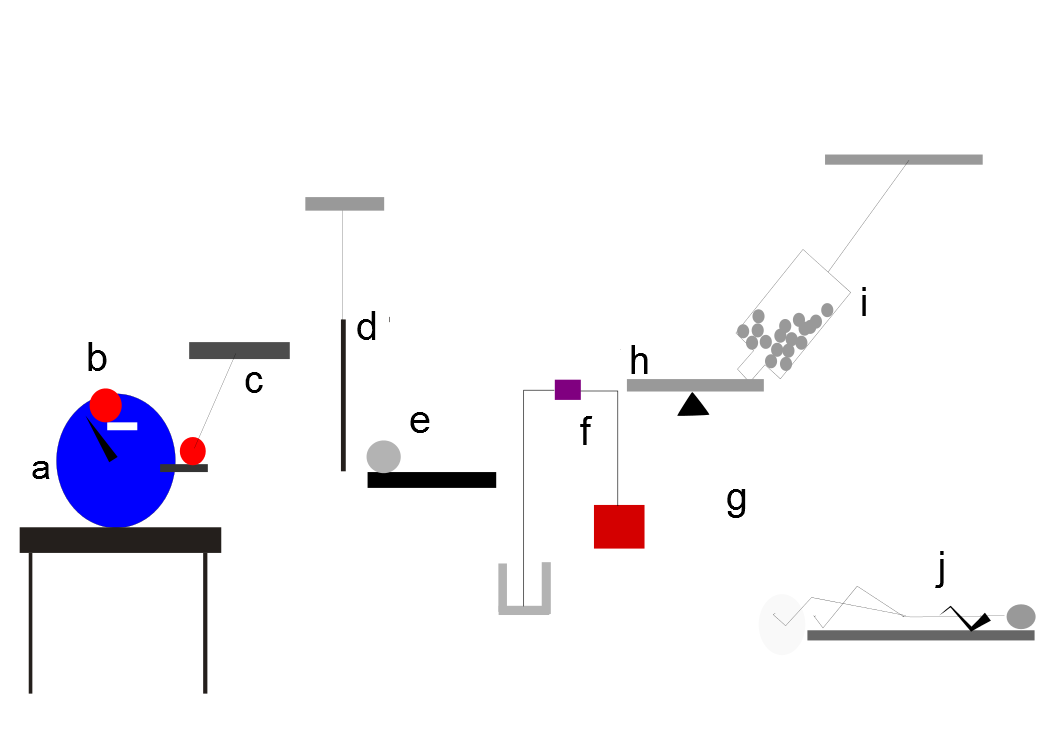
\includegraphics[scale=0.3]{doc/original-design.eps}







\section{Timing Plots}
\section{Plot 1}
\subsection{Loop Time vs Iteration Value} 
Loop time , as one might expect increases with iteration values . However the subtler observation is that the slope of the graph decreases as Iteration value increases after a certain threshold(iteration value around 40 in this case).\\
We could infer that the operating system perhaps allots more resources to the process as the load of the process increases. Since the slope doesn't decrease uniformly , we can say that this happens after a certain threshold load. \\
Also when the data is taken with a loaded system , the values of loop time is slightly higher and its slope is steeper.\\

 \subsection{Average Step Time vs Iteration Values}
Average Step Time decreases with iteration values. The reason is same . The operating systems allots more resources to the process as the load increases.\\
When system is loaded Average step time values are slightly higher. \\
\footnote
  { 
 \begin{enumerate}
   \item 
  The first graph is when the system is unloaded and the second graph is when the system is heavily loaded.
   \item
   Note the differences in scale in graphs . This is because autoscale was used in the scripts.
 \end{enumerate}
 }
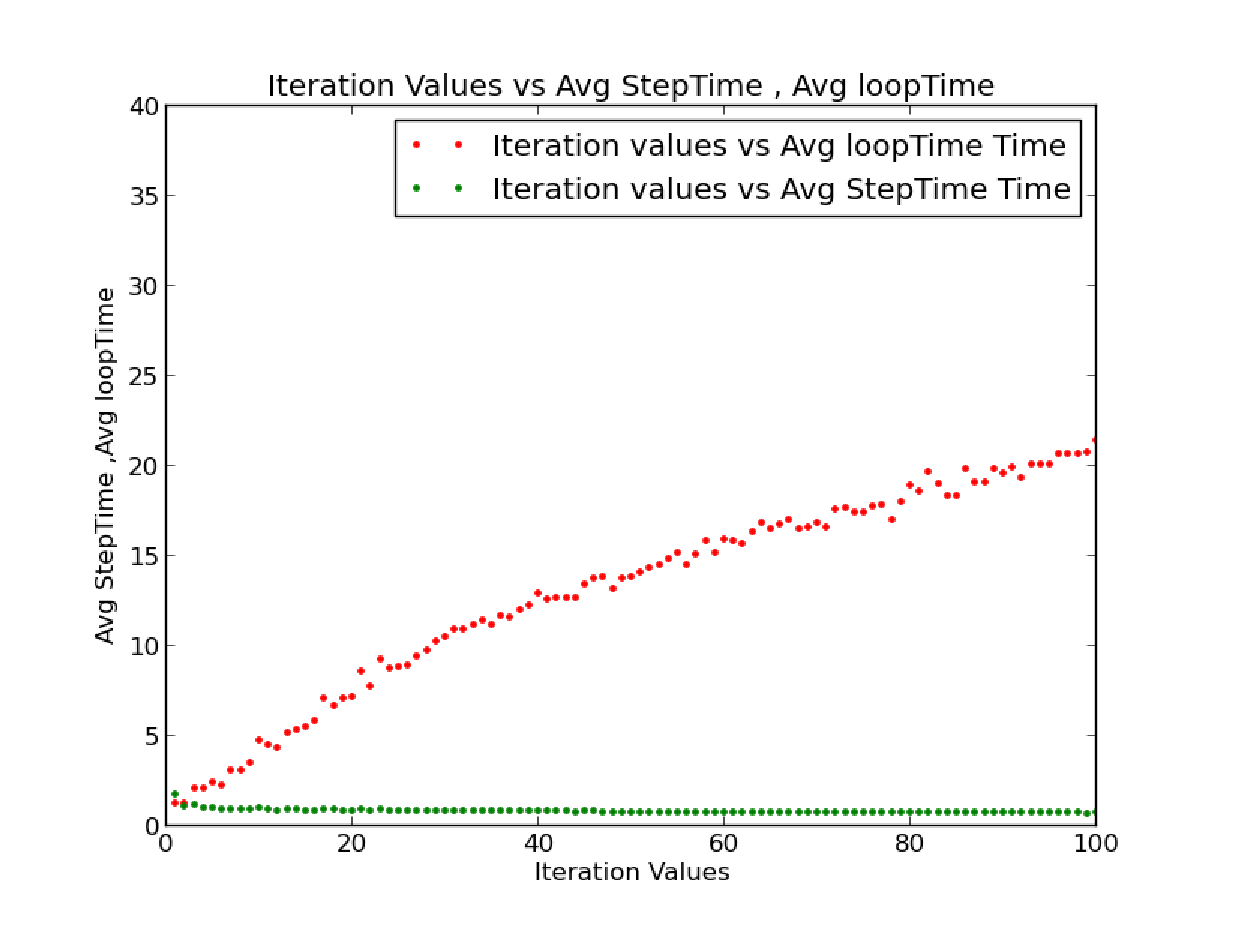
\includegraphics[scale=.3]{doc/g12_plot01.eps}
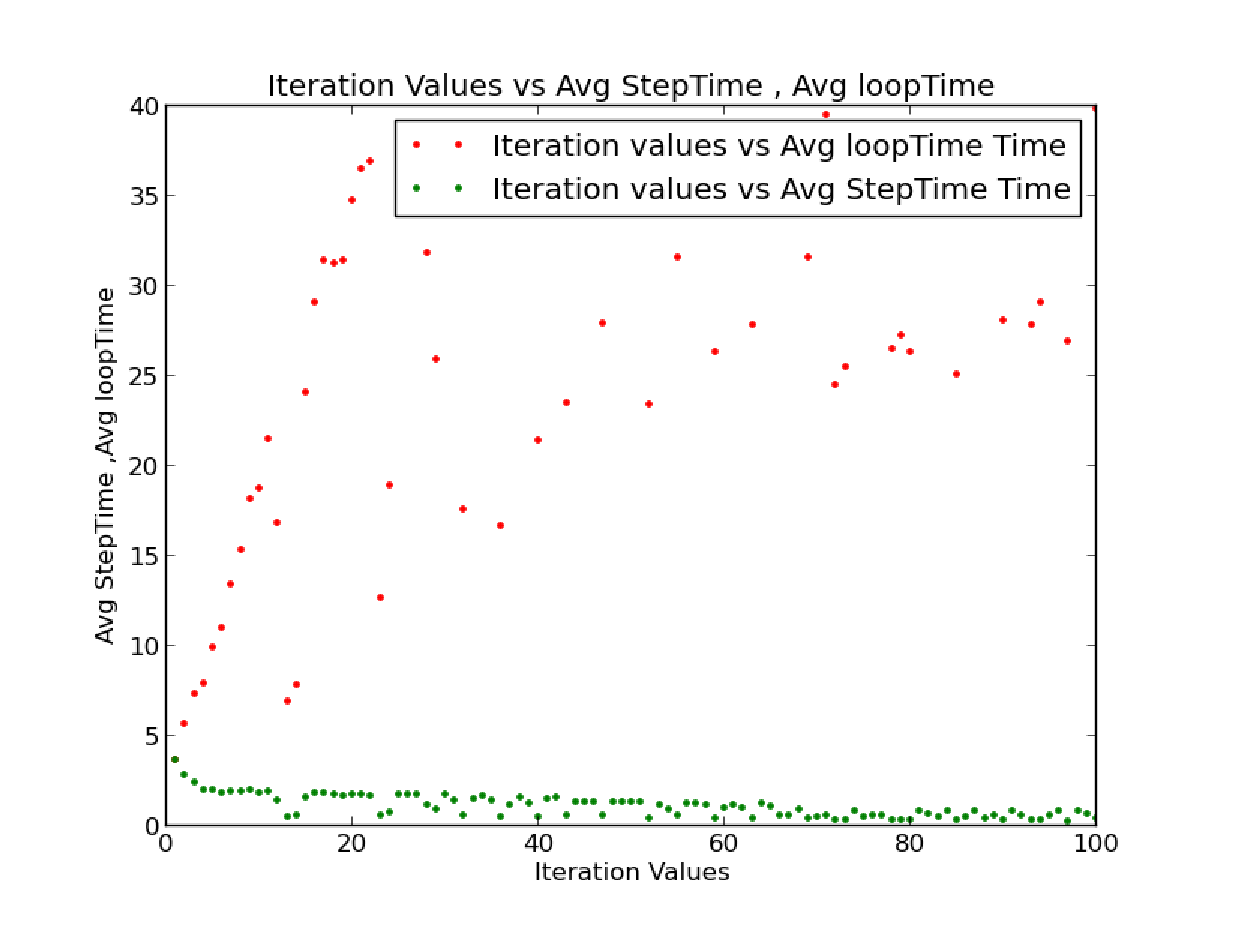
\includegraphics[scale=.3]{doc/g12_plotload01.eps} \\




\section{Plot 2}
\subsection{Quantities Averaged over Rerun values vs Iteration Value} 
All quantities (Step time, Collision time , velocity time and Position time) decrease as iteration value increases.
Again the reason is same . The operating systems allots resources as per the load of the process. Bigger processes are alloted more resources.\\
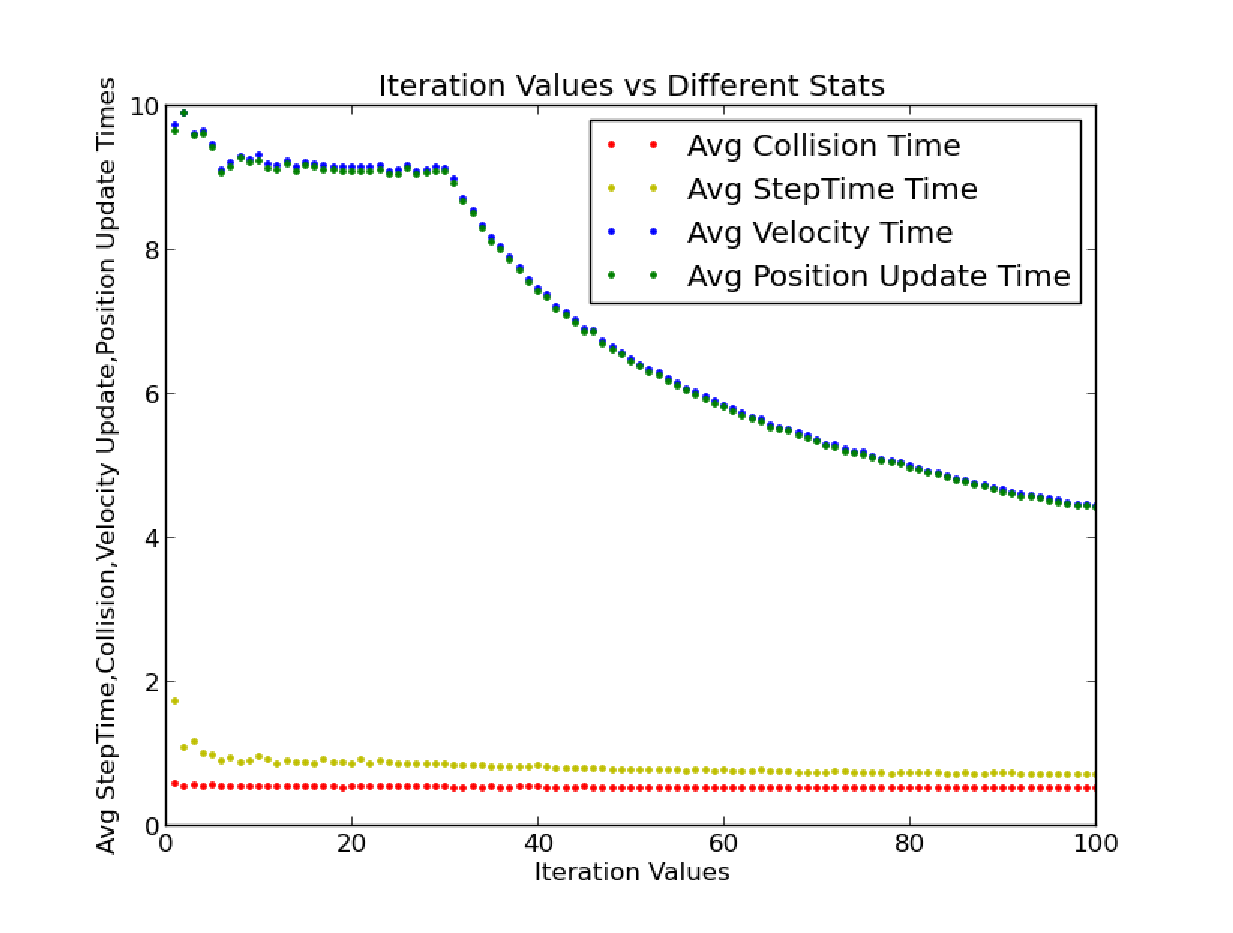
\includegraphics[scale=.3]{doc/g12_plot02.eps}
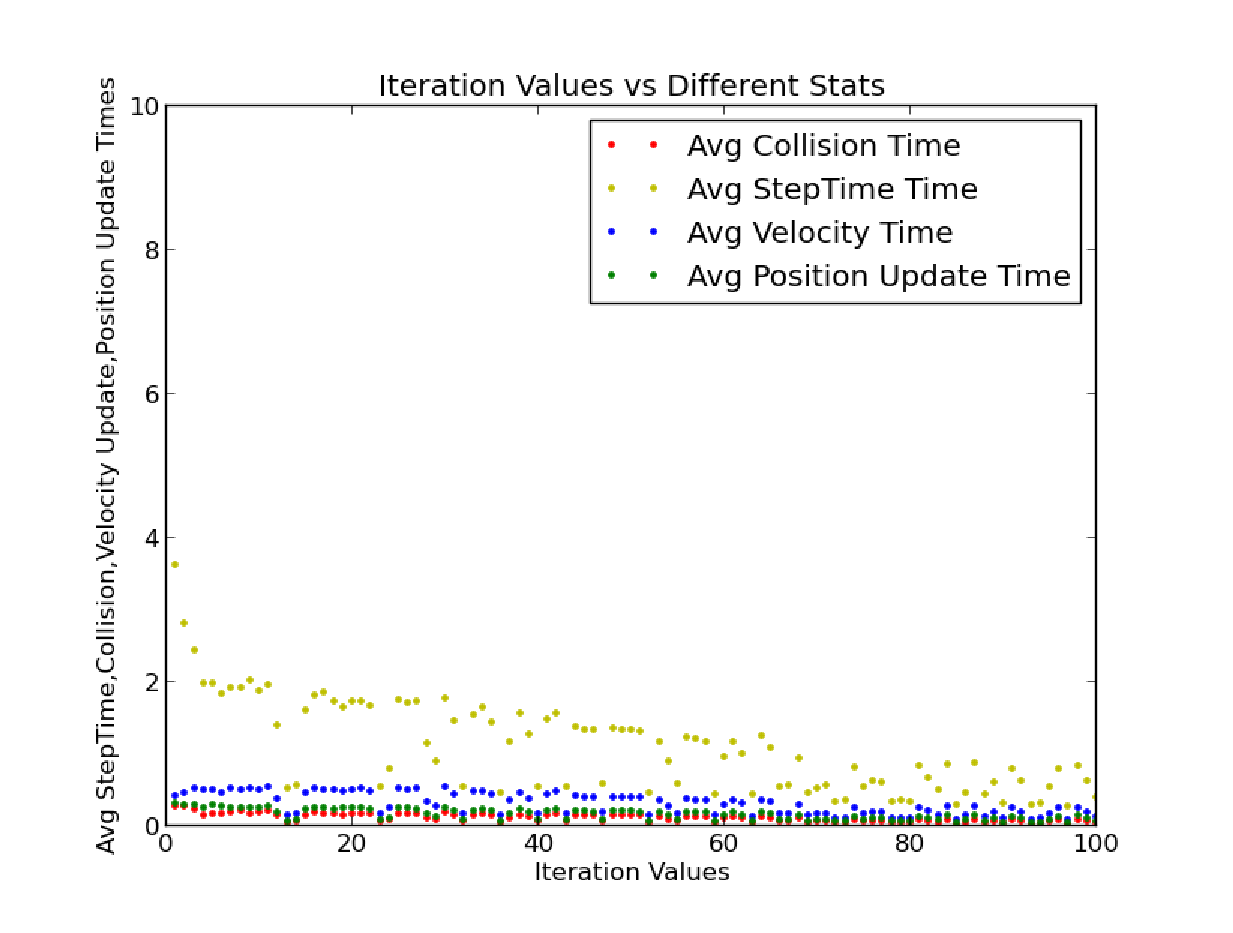
\includegraphics[scale=.3]{doc/g12_plotload02.eps} \\

\section{Plot 3}
\subsection{Average Step Time vs Rerun values ,  Loop Time vs Rerun values} 
Not surprisingly, the graph is more or less horizontal i.e.constant with rerun values. For every rerun value the same set of commands are executed in more or less a similar environment(similar amount of load on the system) and hence this result.\\
when the system is loaded , the graph is still horizontal but the values are slightly higher.

\section{Plot 4}
\subsection{Quantities Averaged over Rerun values vs Rerun Values} 
All quantities (Step time, Collision time , velocity time and Position time) roughly remains constant with rerun values.\\
Again the reason is same . The operating systems executes the same set of commands for each rerun value in a similar environment.\\
when the system is loaded , the graph is still horizontal but the values are slightly higher.\\

\section{Plot 5}
\subsection{Step Time Errorbars vs Iteration Values} 
Step time as discussed for plot 1 , decreases with iteration values. From the plot , we observe that the standard deviation of the Step time errorbars decreases with increase in Iteration values.\\
This is because as the iteration value increases , the number of data points for the calculation of Average step time increases. Consequently the standard deviation decreases on an average.\\
When the system is loaded , the standard deviation  doesn't vary so smoothly. We see more deviation from the characterstic of the graph stated above.\\
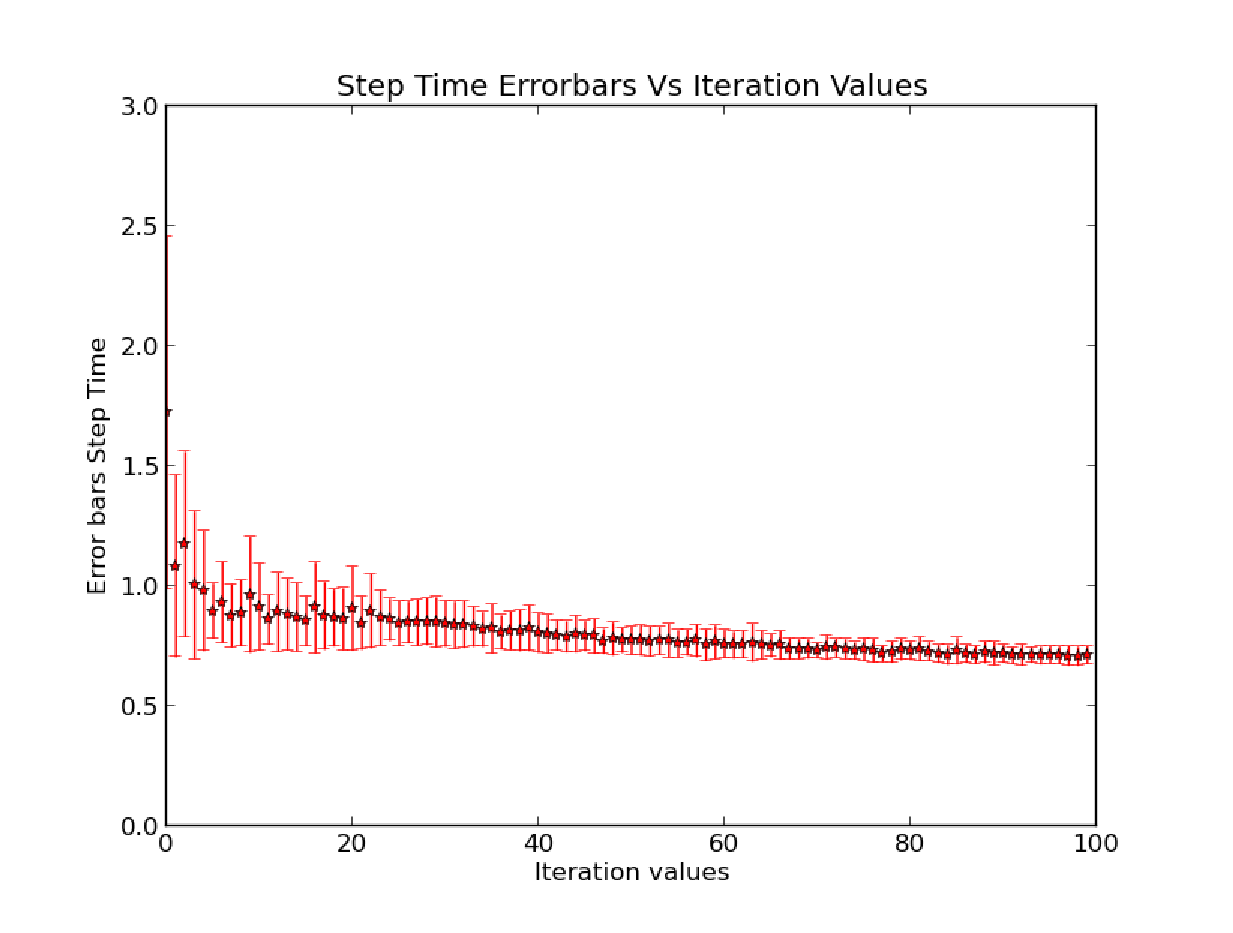
\includegraphics[scale=.3]{doc/g12_plot05.eps}
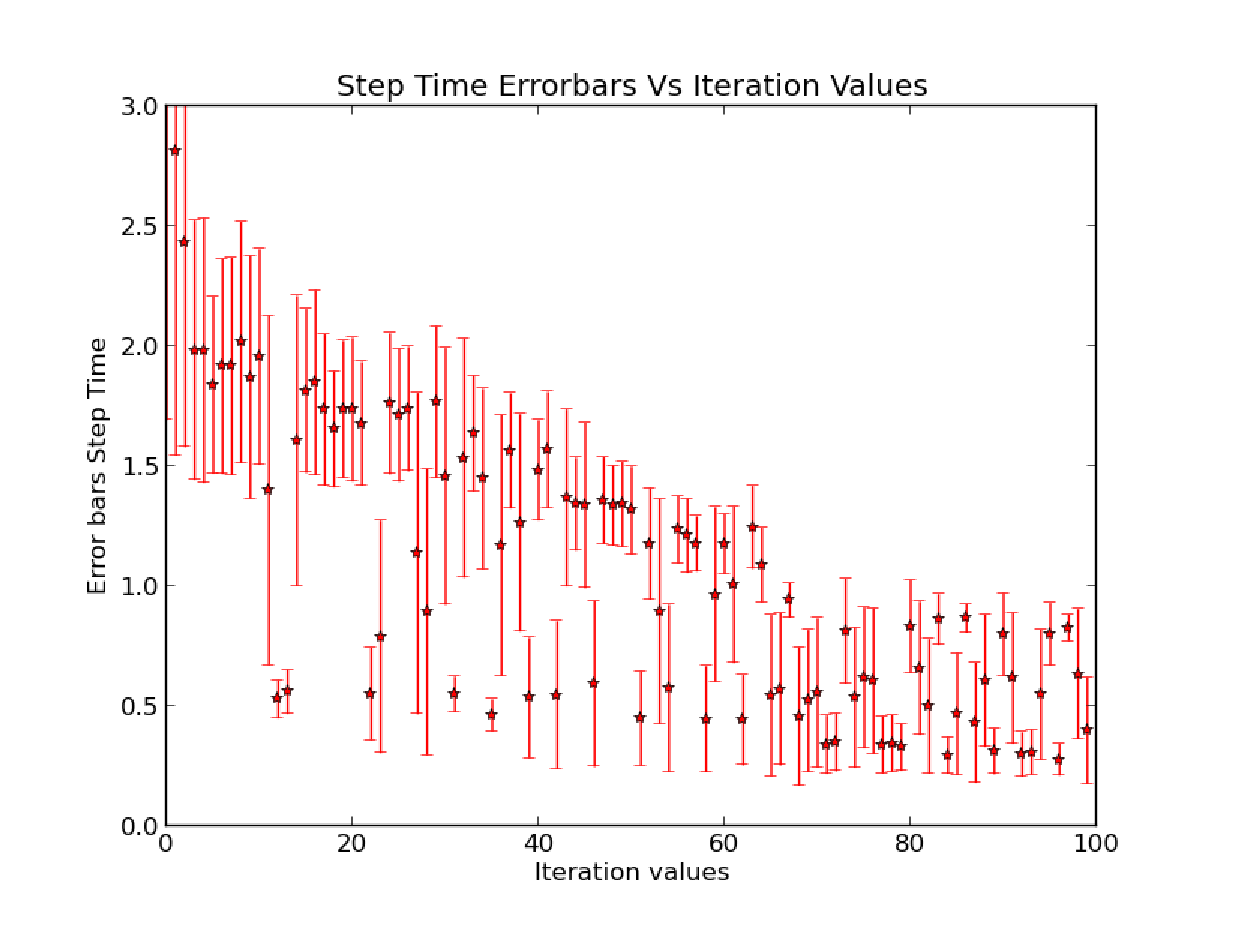
\includegraphics[scale=.3]{doc/g12_plotload05.eps} \\

\section{Plot 6}
\subsection{Cumulative Frequency vs Step Time, Frequency bars bs Step Time} 
The Frequency bars peak at the mean Average Step Time and thus the Cumulative Frequency has the steepest slope around this mean.\\ 
When the system is loaded, the frequency bars are more spread and cumulative frequency has a flater slope around the mean. The value of the mean itself is larger.\\
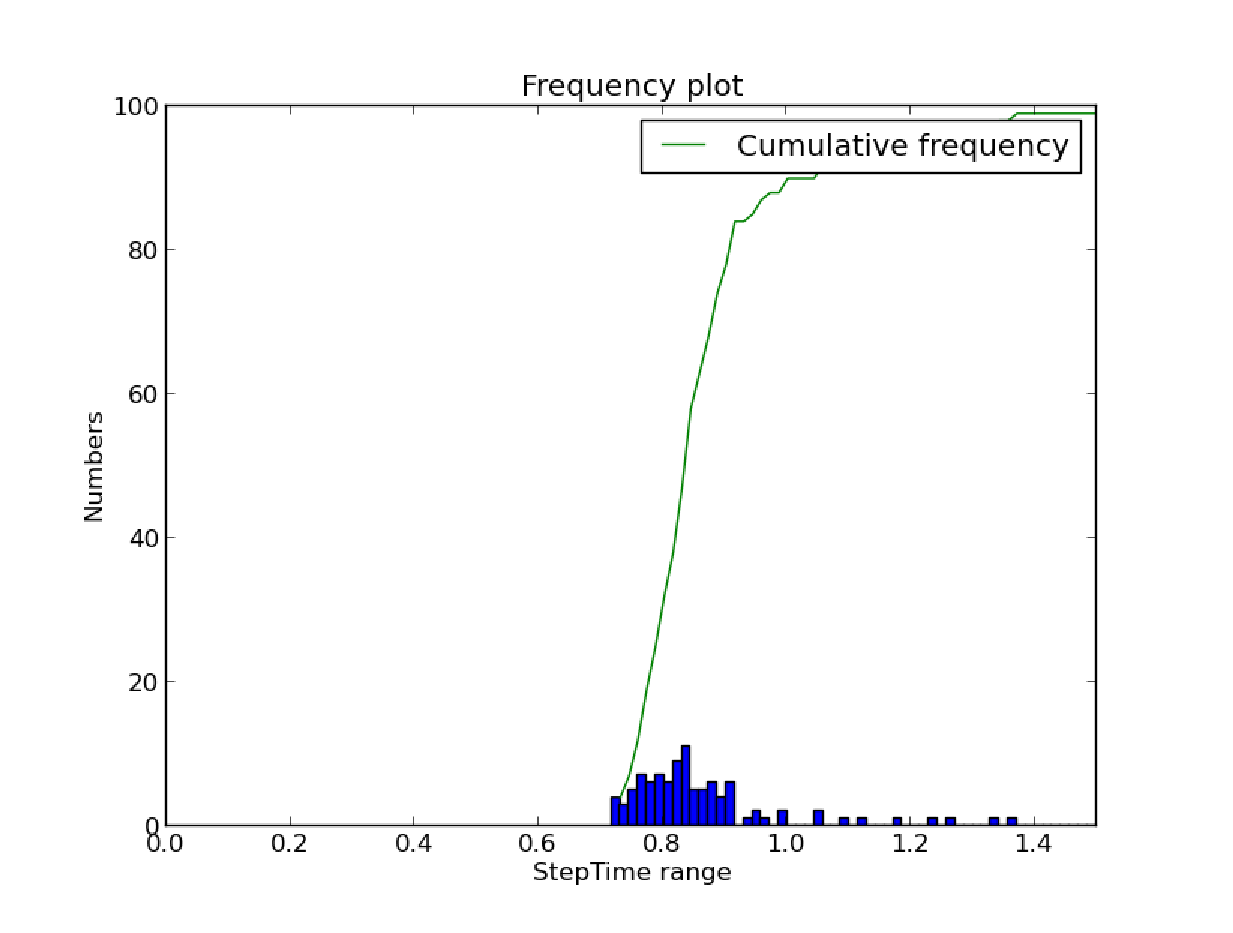
\includegraphics[scale=.3]{doc/g12_plot06.eps}
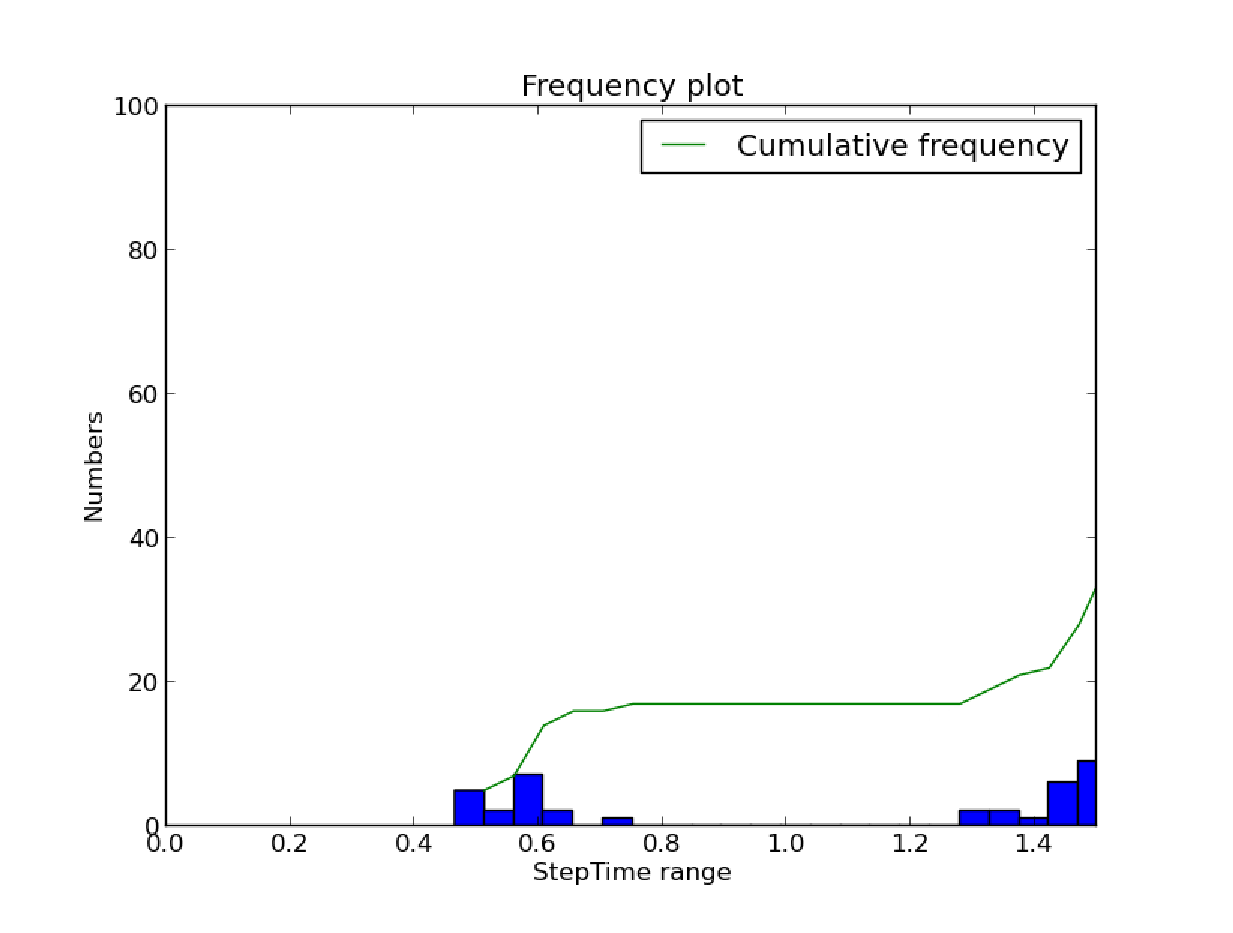
\includegraphics[scale=.3]{doc/g12_plotload06.eps} \\




\section{Profiling Reports}
\subsection{Observations}
From the profiles, we see that
\begin{enumerate}
  \item 
 \textit{b2ContactSolver::SolveVelocityConstraints()} takes the maximum amount of time.
 \item
  The \textit{b2Vec2::b2Vec2(float, float)} is called the maximum number oftimes followed by \textit{operator-(b2Vec2 const, b2Vec2 const)} and \textit{operator*(b2Vec2 const, b2Vec2 const)}. These functions are mostly called from \textit{b2ContactSolver::SolveVelocityConstraints()}.
\end{enumerate}

\subsection{Debug Mode Profiling}
For the Debug mode , all optimization flags(-On) were turned off. Expectedly the time taken was much higher in this case.
There is no optimization and the call-graph is precisely as the structure of the program. We observe that there are some very trivial functions which are called a very large number of times (b2Vec , All b2Vec Operators - (*, + , -) etc).\\
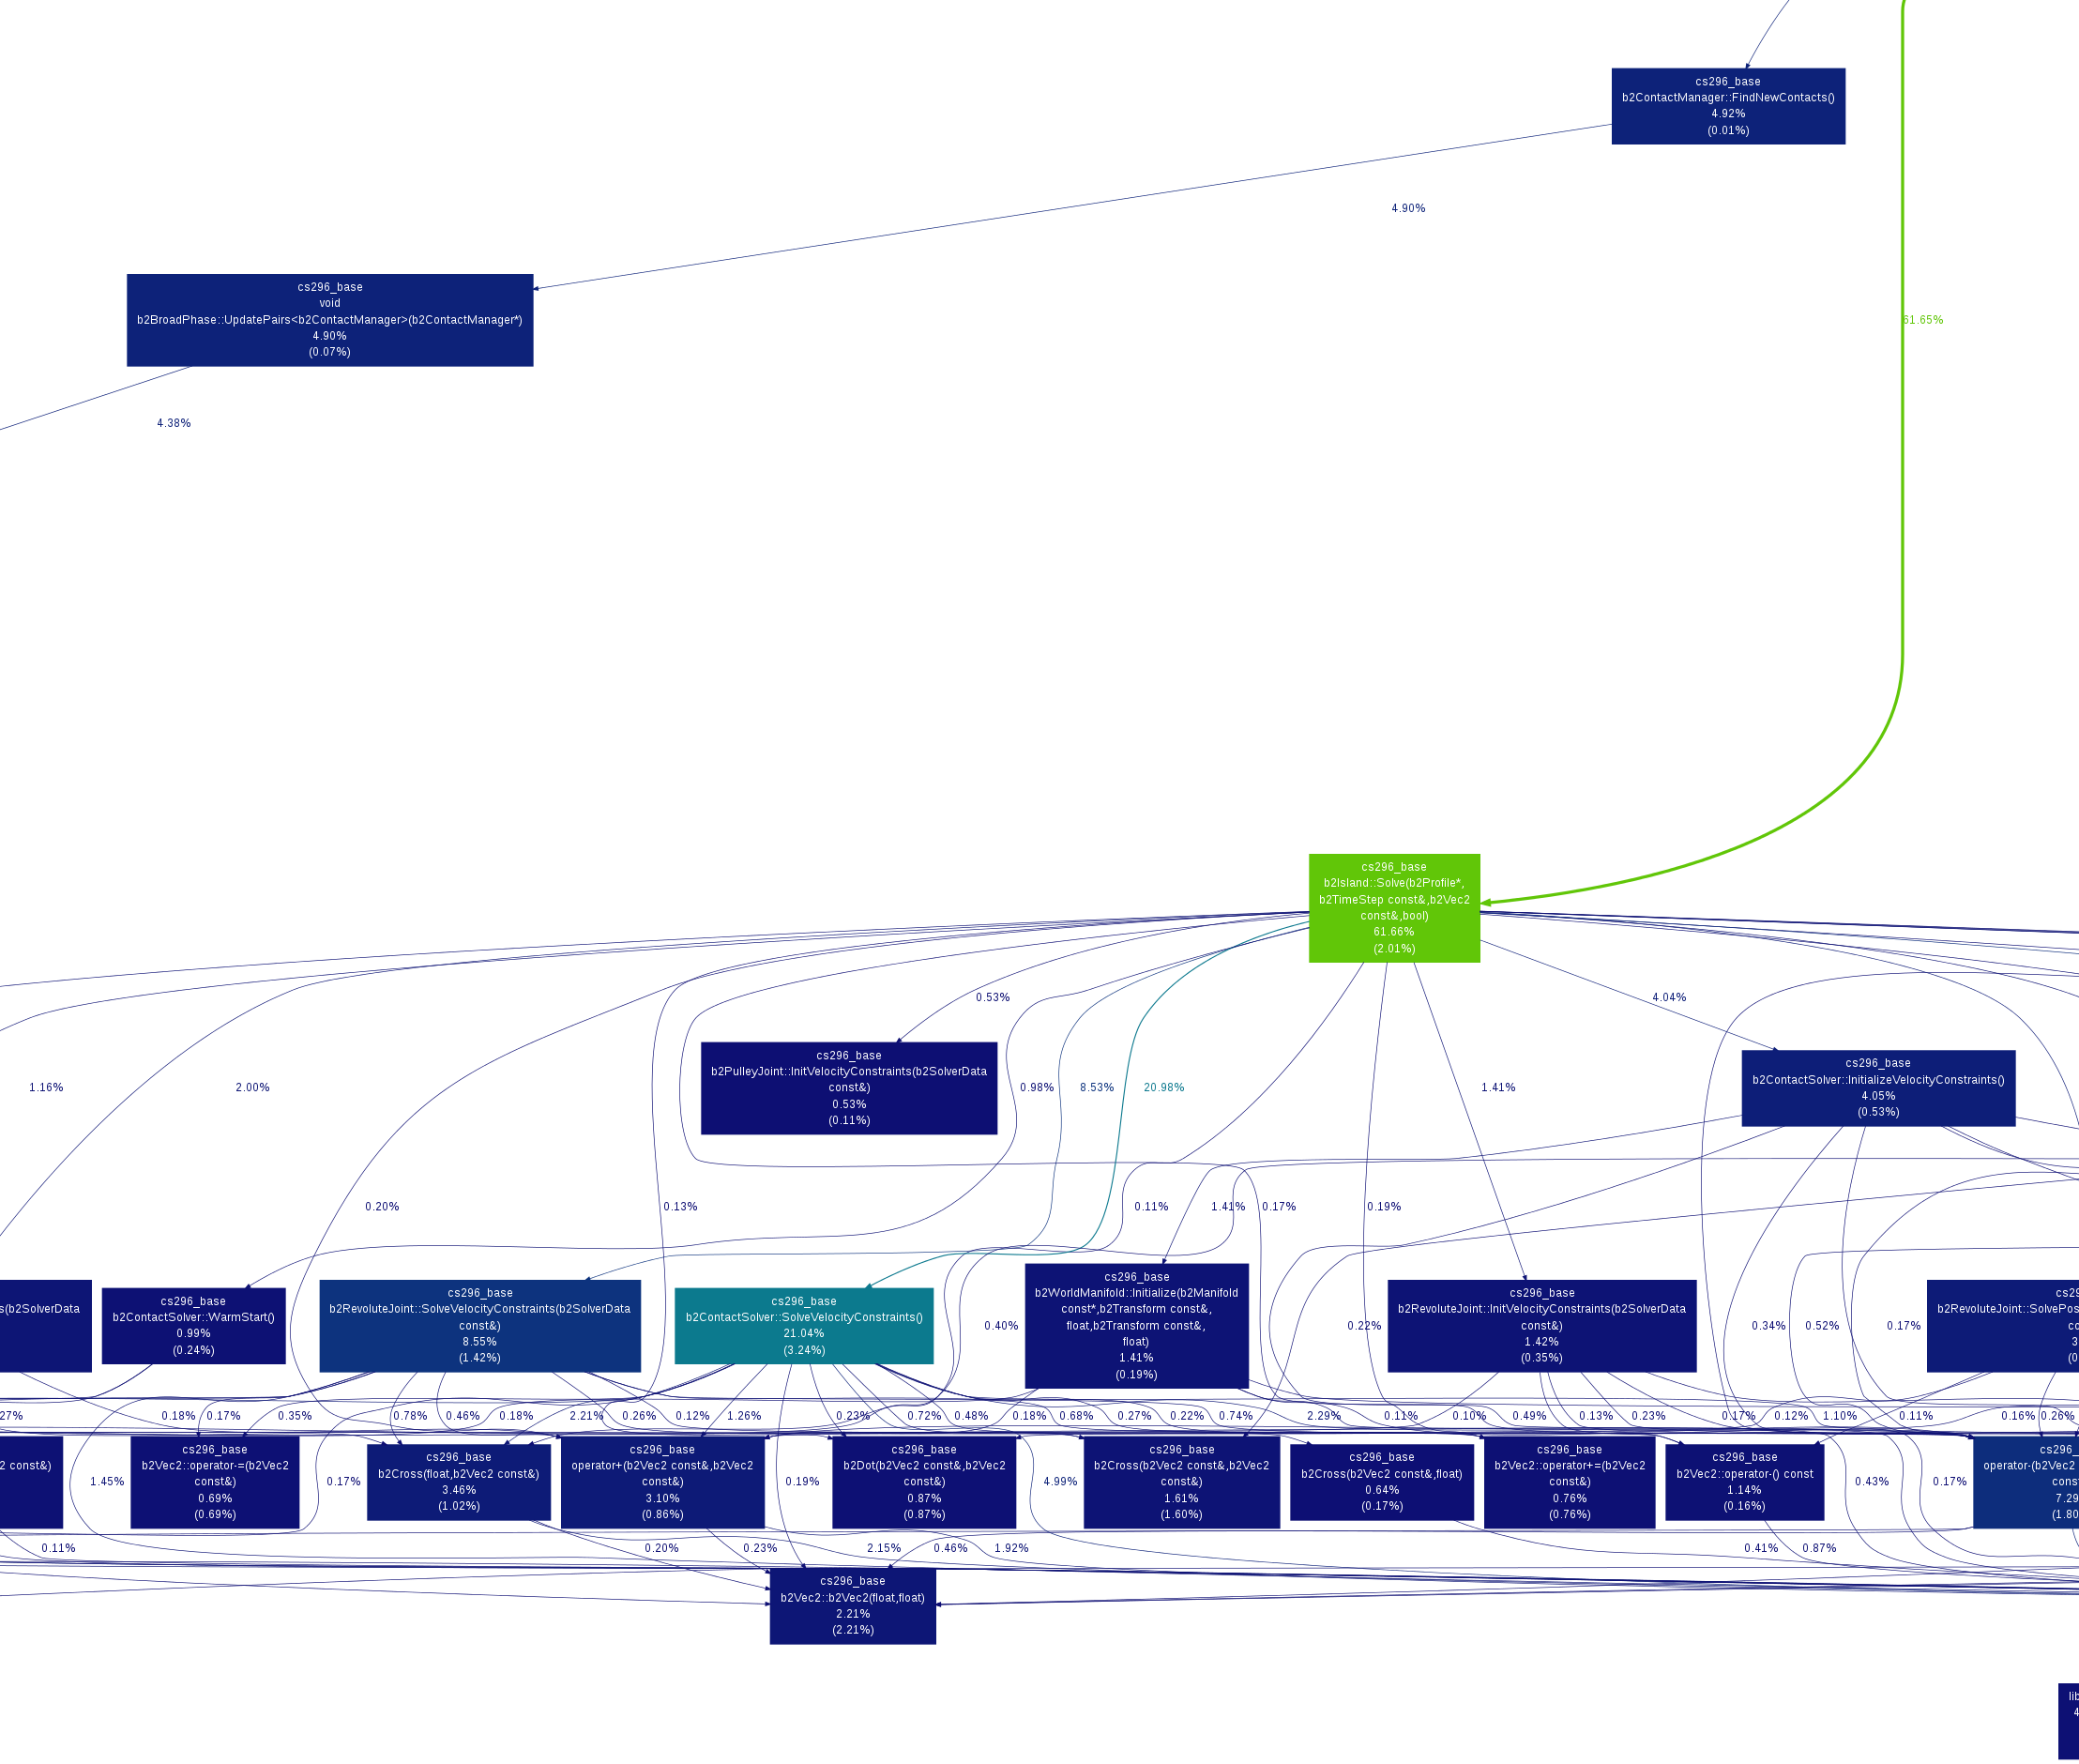
\includegraphics[scale=.2]{doc/debug1.eps}\\
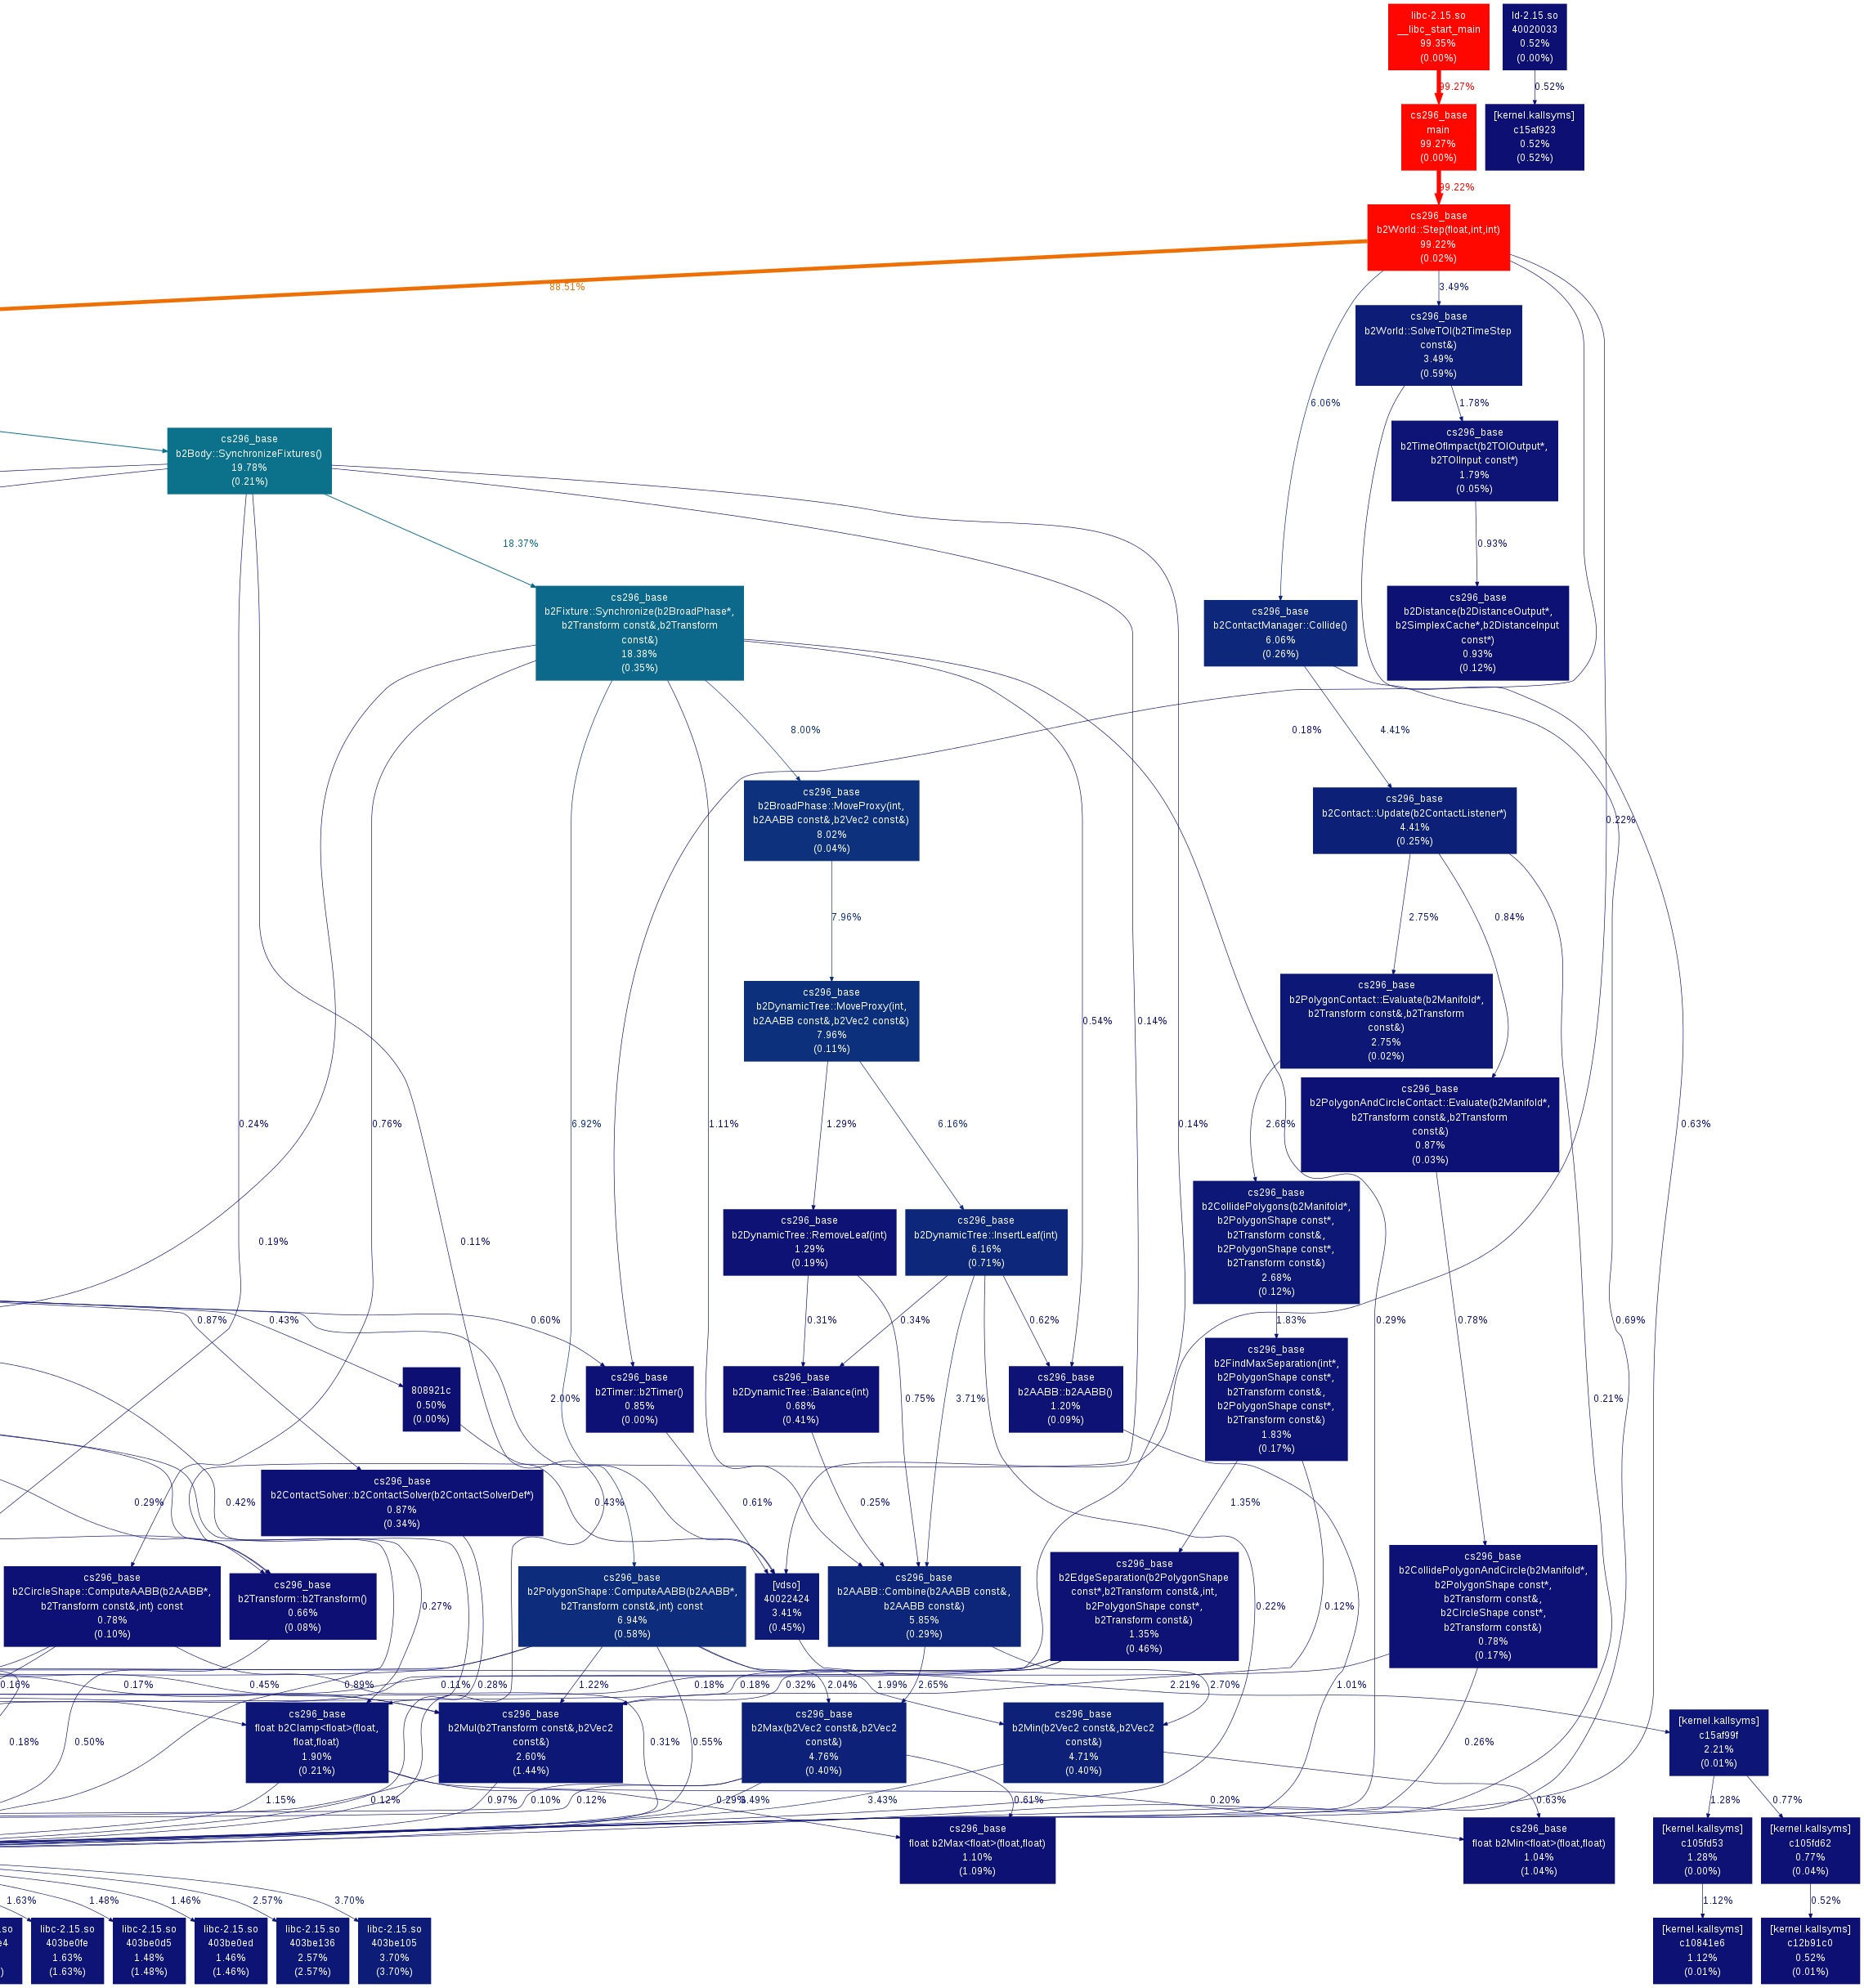
\includegraphics[scale=.2]{doc/debug2.eps} \\

\subsection{Release Mode Profiling}
For the release mode , -O3 optimization flag was turned on. The time taken in this case is significantly less than that taken for the debug mode profiling.\\
The call graph for this case is quite interesting. There is only one level in the tree. There are several functions which are not shown in the tree. This is because most of the inline functions were replaced by their codes by the compiler. This leads to huge improvement in running time because if we carefully observe the call-graph for the debug profiling mode , some of these functions (b2Vec , All b2Vec Operators - (*, + , -) etc) were called more than 10000000 times. As a result the compiler does a lot of redundant work to  retrieve the codes of these inline functions from the function stack without the optimization flag.


There are several other optimizations that the compiler does . Some of these are
\begin{enumerate}
  \item 
Identifies and optimizes tail recursive calls. 
 \item
Optimizes assignment operations(temporary variables) and loop iteration variables 
\end{enumerate}
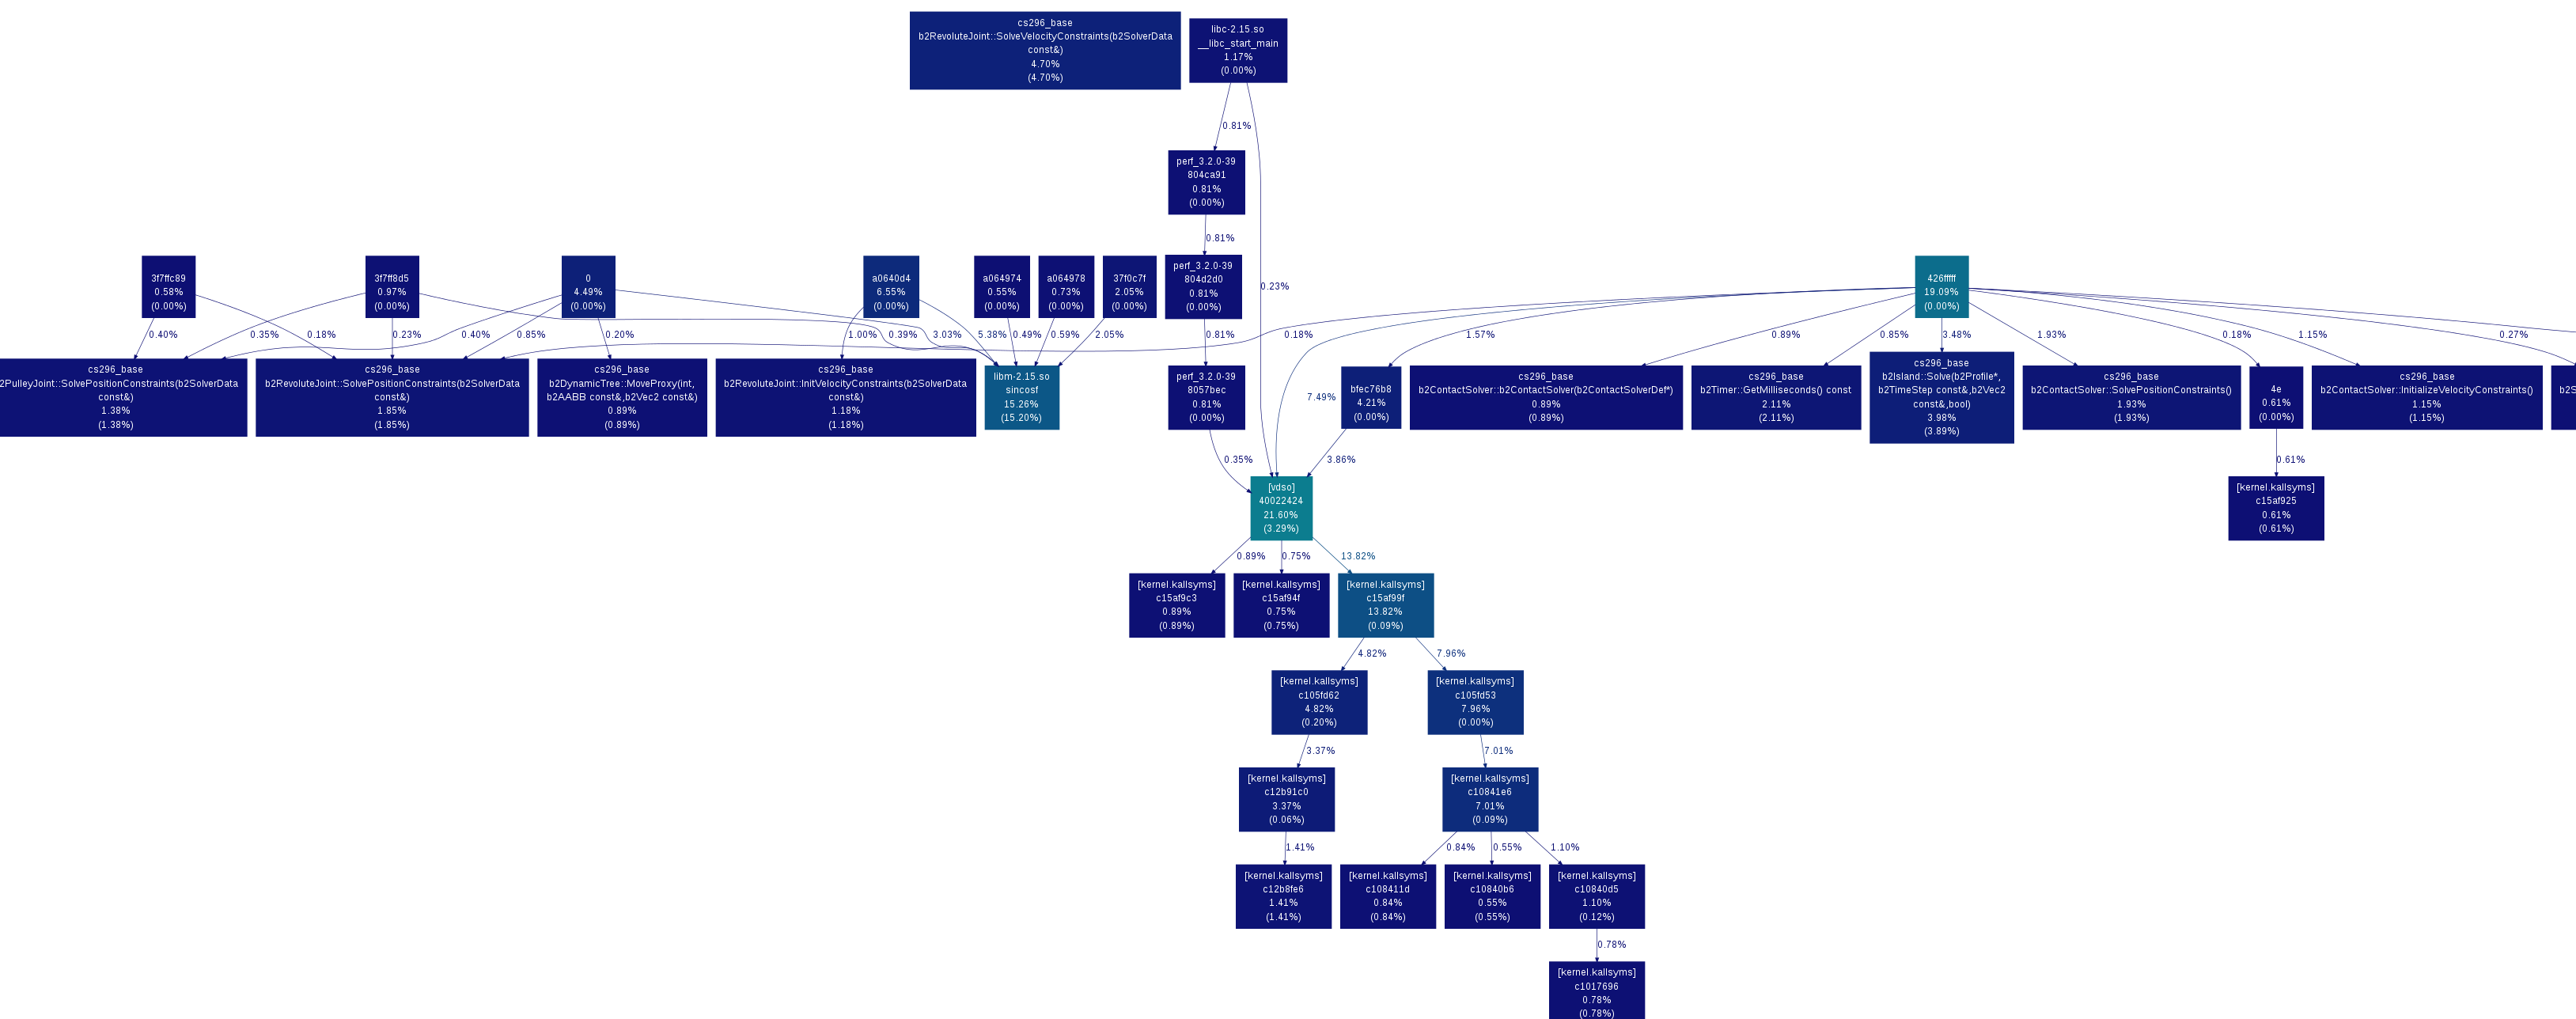
\includegraphics[scale=.2]{doc/release.eps} \\

\nocite{*}
\bibliographystyle{plain}
\bibliography{doc/myrefs}{}
\end{document}
